\section{Methodology}
\label{sec:methodology}

% I'm using the \dataset command to avoid different constructions like "dataset" and "data set" in the text.
\textbf{Data sources.} The core of our analysis uses a \dataset provided by \openintel~\cite{openintel}. \openintel is a large-scale, active DNS measurement platform.
Our goal is to provide a country-level view of \gls{DMARC} adoption along with inter-country relationships between organizational domains and the domains configured to receive and possibly process \gls{DMARC} reports.
We compare government domain names to assess whether they follow \gls{DMARC} guidelines set by their own security agencies (\eg CISA for the U.S. \texttt{gov} domains~\cite{_BOD1801Enhance_2017}).
To achieve our goals, we use \gls{DMARC} data for \gls{ccTLD} domain names, which were derived from \gls{CT} logs\footnote{\url{openintel.nl/data/forward-dns/ctlog-names}}.
Such data derives from \gls{DNS} queries on \texttt{\_dmarc.DOMAIN}, where \texttt{DOMAIN} is the second-level domain name, or so-called organizational domain.
Sommese \etal~\cite{SommeseEtAl_ThisLocalDomain_2024a} showed that domain names derived from \gls{CT} logs account for a substantial part of the full \gls{ccTLD} zone.
We use \gls{CT} logs as a source of domain names to examine \gls{DMARC} adoption and the use of the reporting system at the \gls{ccTLD}-level. The domain names from \gls{CT} logs are extracted from the certificates' Common Names and the Subject Alternative Name extension.
We use 75M unique domain names (from October 2025). The \dataset covers 301 \glspl{ccTLD}. We assume that \gls{ccTLD} domain names target users in the respective country (see the limitations below). The~\cref{fig:methodology} illustrates our data sources and methodology's steps.

\begin{figure}[tb]
    \centering
    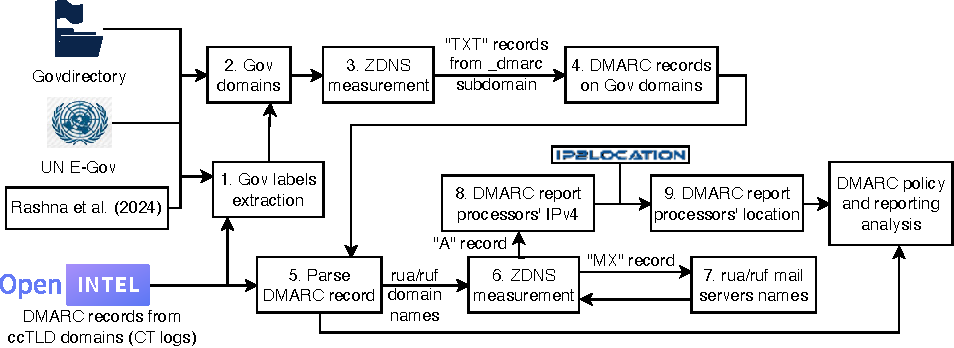
\includegraphics[width=1.\linewidth]{figures/methodology.pdf}
    \caption{Methodology to characterize \gls{DMARC}.}
    \label{fig:methodology}
    \vspace{-15px}
\end{figure}

We extract \gls{DMARC} data from TXT records, as illustrated in step 4 of~\cref{fig:methodology}. We investigate the \texttt{p} (policy) and \texttt{sp} (subpolicy) tags to determine how stringent the domains are with \gls{DMARC}. We also examine the \texttt{rua} and \texttt{ruf} tags to determine where \gls{DMARC} telemetry data is requested to be sent. We analyze \gls{DMARC} strictness of a domain with ``stringent'' and ``permissive'' labels, where ``stringent'' has \texttt{p=quarantine / reject} or, when \texttt{sp} is present, \texttt{sp=quarantine / reject}. Any other configuration we define as ``permissive''.
% subpolicy explained: https://dmarcly.com/blog/how-dmarc-works-with-subdomains-dmarc-sp-tag

To enrich our \dataset, we include GovDirectory~\cite{govdirectory} and United Nations E-Government Knowledgebase~\cite{_EGOVKBUnitedNations_}. The GovDirectory is a curated list of government (and related) domain names worldwide. The UN base lists national and other recognized government portals.

We start with 10,110 unique known governmental domains from 196 countries -- 9,858 domains from 38 countries in GovDirectory and 265 domains from 193 countries in the UN \dataset.
% UN does not have the portals for Bermuda, Greenland, Russia, where govdirectory has them
From this set of known government domains, we learn the labels commonly used for government \gls{TLD} (\eg \texttt{.gov}, \texttt{.gov.ccTLD}) using \textit{publicsuffixlist} (publicsuffix.org), enabling us to identify other government domains in the \openintel data. Identification occurs when the domain names in the government \datasets match those in our \dataset, or when they contain the government labels we extract. The labels we focus on include, with a subset from Rashna \etal~\cite{rashna2024}: \texttt{gov, gv, gc, go, gob, gub, kommune, govt, govern, gouv, government, mil, fed, admin} and \texttt{guv}. In total, we use government domains across 290 countries (step 1).

We make best efforts to identify government domain names. In some cases, due to how regions use the \glspl{TLD}, we may miss domains. For instance, the U.S. uses \texttt{.gov}, Peru uses \texttt{.gob.pe} (derived from the Spanish language), and the Netherlands has no specific \gls{TLD} label for government domains. Hence, our filter finds \texttt{dhs.gov} in the U.S., GovDirectory and the UN \datasets help identify the Peruvian government domain from the label extraction, and we find cases such as \texttt{rijksoverheid.nl} (Dutch government) using the domains already present in the GovDirectory.
% https://publicadministration.un.org/egovkb/Data-Center
% list of .gov: https://en.wikipedia.org/wiki/.gov

\textbf{New measurements.} Some governmental domains in GovDirectory and the UN \dataset are missing from \openintel \dataset. Hence, we use ZDNS~\cite{Izhikevich_ZDNS_A_Fast_2022} to retrieve TXT records from the \texttt{\_dmarc} subdomain of each governmental domain (step 2). Our measurement campaigns are from a \gls{VP} in the Netherlands in October 2025. The measurements provide us with 374 additional governmental domains with \gls{DMARC} data.

To infer indications on how \gls{DMARC} telemetry data is shared across regions, we geolocate the email servers of domains in \texttt{rua} and \texttt{ruf} tags. We extract domain names from the email addresses specified in the \texttt{rua} and \texttt{ruf} tags of \gls{DMARC} data. We use ZDNS to perform \gls{DNS} measurements (step 5). First, we measure the MX record to extract the domain name of the email exchanger to which the \gls{DMARC} policy specifies reports are to be sent (step 6). Then we measure the A records (IPv4 addresses) of the domain name from the email server (step 7). We use \iptwolocation to geolocate the mail exchanger IP addresses (step 8).

\textbf{Longitudinal analysis.} To understand whether countries are improving their anti-spoofing infrastructure, we leverage \openintel's \gls{DMARC} measurements since February 2024. We conduct a longitudinal analysis of \gls{DMARC} adoption and the share of \gls{DMARC} telemetry data. We analyzed \gls{DMARC} policies (\texttt{p} tag) over time for organizational domains in various \glspl{ccTLD} and in governmental domains.
Furthermore, we analyze domain names in \texttt{rua} and \texttt{ruf} tags over time to identify trends of \gls{DMARC} report configured to transmit data across countries (when the organizational domain names' \gls{TLD} is different from the \gls{TLD} in \texttt{rua} and \texttt{ruf} tags).

\textbf{Limitations.}
\gls{CT} logs cover a substantial portion of (59\% on average~\cite{SommeseEtAl_ThisLocalDomain_2024a}), but not all, domain names in \glspl{ccTLD} zone files. Hence, we consider the names learned from logs to be a fair representation of the global \glspl{ccTLD} landscape.

We infer the geographical location of domains based on their corresponding \gls{ccTLD}.
In this context, we assume that domain names with a specific \gls{ccTLD} are primarily associated with the country that the \gls{ccTLD} represents. This assumption is especially relevant for \glspl{ccTLD} with dual meanings (\eg~\texttt{.tv} for Tuvalu, commonly used for television-related sites) or look-alike \gls{TLD}, such as \texttt{.co} (Colombia) being used as shorter alternative for \texttt{.com}~\cite{_ManagingMultiRegionalMultilingual_a}.

While a single \gls{VP} perspective constrains our ability to make definitive global inferences and we do not examine the extent of client-scoped responses~\cite{10.1145/3730977} on MX record resolution, the findings nevertheless demonstrate that DMARC is, in certain instances, configured to transmit data across national borders.

U.S. organizational domains with \gls{DMARC} are underrepresented in our \dataset.
The U.S. domains might be registered under, \eg \texttt{.com} or other \glspl{gTLD} for historical reasons.

We do not measure \gls{EDV} on \gls{DMARC} reporting because only a few \glspl{ESP} actually perform \gls{EDV} checks~\cite{hureau_stress_testing}.
Hence, \glspl{ESP} may send reports to external domains even when the required configuration is missing.
Therefore, we treat these cases as instances of \gls{DMARC} telemetry configured to be transmitted across domains.
%As a result, our measurements represent an upper bound on the number of domains that share DMARC telemetry data externally.

Finally, we don't scan subdomains to capture when policy override occurs, \ie when another policy \texttt{p} is defined in a subdomain which takes precedence over the main domain policy.
Subdomain policies have been studied~\cite{MaroofiEtAl_AdoptionEmailAntiSpoofing_2021}, and our goal is not to characterize the policy distribution, but to give an overview of domains in \glspl{ccTLD} stringency using \gls{DMARC}.
% I cannot estimate the impact of scanning subdomains because Maroofi et al. do not specify how many subdomains they found with a DMARC policy. They use the TOP500 domains in their scan, and Table IV shows domains specific without SPF records and subdomains without DMARC. But this limitation is worth mentioning.

\begin{table}[tb]
\scriptsize
\centering
\caption{Overview of our \dataset. All ccTLDs and the government-related domains.}
\begin{tabular}{lr}
\toprule
    & Total \\
\hline
Domains using DMARC & 19.2M \\
\ldots \# ccTLDs & 301 \\
\ldots \# countries & 290 \\
\ldots with either \texttt{rua} or \texttt{ruf} & 5.8M \\
\ldots \ldots with \texttt{rua} & 5.7M \\
\ldots \ldots with \texttt{ruf} & 1.9M \\
\hline
Government-related domains using DMARC & 40.0k\\
\ldots \# ccTLDs & 192 \\
\ldots \# countries & 183 \\
\ldots with either \texttt{rua} or \texttt{ruf} & 22.4k \\
\ldots \ldots with \texttt{rua} & 22.1k \\
\ldots \ldots with \texttt{ruf} & 13.5k \\
\bottomrule
\end{tabular}
\label{tab:data_overview}
\vspace{-10px}
\end{table}

\begin{table}[tb]
\scriptsize
\centering
\caption{DNS measurements overview. Measurement steps reffers to~\cref{fig:methodology}.}
\label{tab:dns_meas_overview}
\begin{tabular}{lrrr}
\toprule
\textbf{Step from~\cref{fig:methodology}} & \textbf{Step 3} & \textbf{Step 6} & \textbf{Step 7} \\
\midrule
Measurement date & Sep-30 & Oct-10 & Oct-11 \\
\midrule
Total & 10.1k & 1.8M & 1.1M \\
\midrule
NOERROR & 5,798 & 1,726,854 & 1,013,738 \\
NXDOMAIN & 3,989 & 29,287 & 43,763 \\
TIMEOUT & 231 & 58,052 & 894 \\
SERVFAIL & 93 & 886 & 206 \\
ERROR & 0 & 416 & 0 \\
\bottomrule
\end{tabular}
\vspace{-15px}
\end{table}
\textbf{Data overview.}
We summarize the \gls{DMARC} data from \openintel in~\cref{tab:data_overview}.
From all domains in the \dataset, 19.2M (25.7\%) have \gls{DMARC} (\texttt{v=DMARC1}) records. Prior work showed adoption rates of 5.4\% ($\approx$15M) in 2023~\cite{hureau_spoofed}.
% In Table 3 of the previous work, 5.4% of 280M domains is approximately 15M.
We find 5.8M (30\%) of domains with \gls{DMARC} records have either a \texttt{rua} or \texttt{ruf} tag. This contrasts with prior work~\cite{hureau_spoofed}, which found 6.7M (42\%).
Our numbers differ because we focus on \gls{ccTLD} domains, whereas previous work uses a broader \dataset aggregation.
We find 5.2k (51.1\%) government domains with \gls{DMARC} record.
% We don't have a count of gov domains without DMARC in OpenINTEL, so I can't provide a complete view of gov domains with DMARC. Which implies I cannot give numbers in Table Vb.

We provide in~\cref{tab:dns_meas_overview} an overview of our \gls{DNS} measurement campaign. Our ZDNS measurements returned different error codes: a) NOERROR when the query was successful, b) NXDOMAIN when the domain name is absent in the DNS zone file of the queried name server, c) TIMEOUT in the domain name resolution, d) SERVFAIL and ERROR for other errors in the domain name resolution. We observe a high number of NXDOMAIN responses from governmental domains. The NXDOMAIN (step 3) indicates the absence of a \gls{DMARC} record for governmental domains.
%We performed a follow-up DNS measurement on the NS records to determine whether the domains have DNS infrastructure. 3.7k of the NXDOMAIN responses have NOERROR. Hence, the subdomain \texttt{\_dmarc} is not configured for those governmental domains.
% NXDOMAIN (39.5\%).
